 %%%%%%%%%%%%%%%%%%%%%%%%%%%%%%%%%%%%%%%%%%%%%%%%%%%%%%%%%%%%%%%%%%%%%%%%
% Doc class%%%%%%%%%%%%%%%%%%%%%%%%%%%%%%%%%%%%%%%%%%%%%%%%%%%%%%%%%%%%%
%%%%%%%%%%%%%%%%%%%%%%%%%%%%%%%%%%%%%%%%%%%%%%%%%%%%%%%%%%%%%%%%%%%%%%%%
\documentclass[a4paper]{jpconf}

\usepackage{graphicx}
\usepackage{booktabs}
\usepackage{siunitx}
\usepackage{enumitem}
\usepackage[utf8]{inputenc}
\usepackage{csquotes}


\usepackage{subfig,multicol}
\usepackage[export]{adjustbox}
\usepackage{float}

\usepackage[english]{babel}
\usepackage{fancyhdr}

% Page numbers
\usepackage{lastpage}
\pagestyle{fancy}
\fancyhf{}
\rfoot{Page \thepage \hspace{1pt} of \pageref{LastPage}}

% Biber-Biblatex and its configuration
\usepackage[backend=biber,style=authoryear]{biblatex}
\addbibresource{Congested.bib}
%\nocite{*}

% The length of a full paper is limited to 8 pages 
% Deadline for submitting a full paper is 9th January 2020 h. 23.59 CET. 



%%%%%%%%%%%%%%%%%%%%%%%%%%%%%%%%%%%%%%%%%%%%%%%%%%%%%%%%%%%%%%%%%%%%%%%%
\begin{document}
	\title{Mapping the spatial distribution of urban traffic congestion: methodological exploration using web based services }
	\author{Jonathan Cohen and Jorge Gil}
	\address{Department of Architecture and Civil Engineering, Chalmers University of Technology, Sven Hultins gata 6, SE-412 96, Göteborg, Sweden}
	\ead{jonathan.cohen@chalmers.se}
	
	%%%%%%%%%%%%%%%%%%%%%%%%%%%%%%%%%%%%%%%%%%%%%%%%%%%%%%%%%%%%%%%%%%%%%%%%
	\begin{abstract}%%%%%%%%%%%%%%%%%%%%%%%%%%%%%%%%%%%%%%%%%%%%%%%%%%%%%%%%
		%%%%%%%%%%%%%%%%%%%%%%%%%%%%%%%%%%%%%%%%%%%%%%%%%%%%%%%%%%%%%%%%%%%%%%%%
		Sustainable transport systems are a necessary requirement to achieve efficient economic performance, enhance urban quality of life and diminish environmental costs. Congestion, a negative externality of mobility, is responsible for urban pollution, inefficiency and has adverse effects over individuals facing this problem. For these reasons, transport and city planning agencies have developed interests in defining and measuring transportation congestion. Although, different definitions and metrics have been used, congestion measurements are found aggregated at a city level or for particular road segments. This study proposes a methodology that produces information from a web traffic service to map traffic congestion within an urban area. The method is simple and generalizable enough to be adopted in different urban areas. This paper presents the analysis of four European cities (Amsertdam, Glasgow, Goteborg and Lisbon) and show that the conclusions are consistent with the results obtained from internationally recognized organizations such as INRIX and TomTom.
	\end{abstract}
	
	
	%%%%%%%%%%%%%%%%%%%%%%%%%%%%%%%%%%%%%%%%%%%%%%%%%%%%%%%%%%%%%%%%%%%%%%%%
	\section{Introduction}%%%%%%%%%%%%%%%%%%%%%%%%%%%%%%%%%%%%%%%%%%%%%%%%%%
	%%%%%%%%%%%%%%%%%%%%%%%%%%%%%%%%%%%%%%%%%%%%%%%%%%%%%%%%%%%%%%%%%%%%%%%%
	In 2015, global leaders agreed to work towards the 2030 Agenda for Sustainable Development. A total of 18 Sustainable Development Goals (SDGs) were identified as the blueprint for development. The importance of transport to achieve these goals can be direct or indirect, and transportation related indicators are found in eight of these goals (direct: 3.6, 7.3, 9.1, 11.2 \& 12.c and indirect: 2.3, 3.9, 6.1, 11.6, 12.3, 13.1 \& 13.2) \parencite{Booth2000, UN-Habitat2015}. \par
	Sustainable transport systems are acknowledged to be necessary pre-conditions to enhance socio-economic opportunities, diminish environmental costs and improve road safety conditions \parencite{Jennings2016}.\par
	
	By 2030, United Nations projected that urban areas will host 60\% of the global population, within cities over 80\% of the total wealth is being produced \parencite{McKinseyGlobalInstitute2011,UN2018} and the positive externalities associated with urbanity have been extensible registered. Cities are successful because at their core, places of intense human interactions, allowing people to connect easily \parencite{Glaeser2011}. Consequently, the success of cities cannot be explained without the fundamental role of mobility \parencite{Diakaki2003}. However, as cities become more attractive, population density increases and a set of negative externalities such as pollution, crime and congestion erode the benefits of urban life \parencite{Eurostat2016, sdgs2016, Jones1992, Glaeser2011, Stempfel2016}. Nevertheless, traffic congestion is a major urban problem \parencite{Downs1992} because it affects cities' core ability to connect people to other people which is a crucial factor for social and economic development \parencite{Falcocchio2015}. \par
	
	In the last century, cities all over the world have been facing a constant increase in the demand for transportation services, resulting in severe traffic congestion. The future does not look promising, nothing indicates that the situation will get any better. A survey to transportation professionals in \textcite{Bertini2005} shows that almost 80\% believe that congestion problems has worsen. If nothing is done, as a result of congestion travel time, energy consumption and environmental cost will continue rising if \parencite{Bull2004, Diakaki2003}. According to conservative estimates the benefits of increasing the travel speed of private cars by 1 km/h and public transport by 0.5 km/h are worth 0.1\% of the Gross Domestic Product (GDP) \parencite{Thomson2000}.\par
	
	There is an extensive amount of research that has been quantifying the negative impacts of traffic congestion, the \textcite{EuropeanCommission2001} alert that Europe might lose economic competitiveness if no actions are taken to address the problem. The external costs of road traffic were estimated to increase by 80 billion EUR (1\% of the EU GDP). In a similar note, \textcite{Cervero1998, TheTexasA&MTransportationInstitute2019, Lomax1997} argues that these social costs are equal to 2-3\% of GDP and \textcite{Schrank2011} arrives to similar conclusions for the U.S. 
	
	In a more comprehensive attempt, \textcite{Bilbao-ubillos2008} decomposes the costs of congestion into eight categories and provide a detailed methodological tool to quantify the total welfare loss and \textcite{Choi2013} show demonstrate for the U.S. that commuting time have a negative effect in the well-being. Finally, under congested scenarios drivers levels of stress and aggression tend to rise, increasing the probability of unsafe driving \parencite{Hennessy199}.
	
	Significant amount of resources are allocated to understand and measure traffic within cities, decrease in technological costs and fast adoption of mobile devices introduce the possibility of collecting, analyzing and modelling traffic congestion on a wider and more precise scale that in the past \parencite{Rempe2016}. In the past 10 years new information sources and techniques were explored. Cameras and sensors can provide accurate measurements, but only specific road segments are evaluated and the cost of maintaining these devices is high. Alternative methods to collect data at large scale and lower cost is needed\parencite{Pongpaibool2007, Wang2015, Pattara-atikom2006}.\par
	
	
	%\subsection{Research Aim}%%%%%%%%%%%%%%%%%%%%%%%%%%%%%%%%%%%%%%%%%%%%%%%
	%%%%%%%%%%%%%%%%%%%%%%%%%%%%%%%%%%%%%%%%%%%%%%%%%%%%%%%%%%%%%%%%%%%%%%%%
	%As mentioned above, traffic congestion is an urban problem that deteriorate the positive benefits of urban life, %therefore is imperative to understand the problem in depth and look at it from different angles. Traditional %congestion measurements are found to be costly and through practice or research different methods have been explored %to overcome this issue. \par
	
	%One avenue of research understands congestion as a time and location specific problem, which occurs in a road %segment and that its consequences are suffered from those in the immediate surroundings. A second understanding of %the problem deals with the individuals who are affected by traffic. \par
	
	The aim of this research is to provide a methodology to measure how congestion is distributed across an urban area. The map of congestion can provide useful information to local authorities and planners since more dis-aggregated spatial information will be provided. \par
	
	
	%%%%%%%%%%%%%%%%%%%%%%%%%%%%%%%%%%%%%%%%%%%%%%%%%%%%%%%%%%%%%%%%%%%%%%%%
	\section{Theoretical Background} %%%%%%%%%%%%%%%%%%%%%%%%%%%%%%%%%%%%%%%
	%%%%%%%%%%%%%%%%%%%%%%%%%%%%%%%%%%%%%%%%%%%%%%%%%%%%%%%%%%%%%%%%%%%%%%%%
	
	\subsection{What is congestion}
	The definition of congestion in transportation facilities has evolved over the years \parencite{Falcocchio2015} and there is no universal accepted definition for the problem. According to \textcite{Lomax1997}, different actors are interested in understanding different aspects of the problem traffic congestion; hence depending on the what the objective of the study is, different definitions can be adopted, impacting in what metrics are being used and what information is needed to be collected \parencite{Aftabuzzaman2007}. In fact, \textcite{Bertini2005} shows that in practice the definition of congestion is a contested arena, with no clear predominance of one over the other. Time, speed, volume of vehicles, level of service (LOS) and cycle failure are among the most used components to define congestion. \par
	In some cases the definition of congestion is confused with the consequences it produces. \textcite{Aftabuzzaman2007}, proposes to categorize the definitions in 3 groups: (i) demand capacity related, (ii) delay-travel time related, and (iii) cost related. But in the second and third cases, congestion is defined by its outputs and this is found conceptually inaccurate. \par 
	Traffic engineers would define congestion as a situation (without a negative connotation) produced when the amount of infrastructure users exceeds it's capacity. The overuse of the infrastructure results in a set of side effects \parencite{Diakaki2003}. According to \textcite{Falcocchio2015}, 
	to be helpful in congestion management decisions, the definition should be based on a comparison of “actual travel times” with “expected travel times” for peak hour and off-peak conditions. \par
	This idea is rejected by \textcite{Downs1992, JoeCortright2010}, arguing that estimation strategies based on \textit{'inescapable'} travel decisions are  misleading. The \textit{'hypothetical alternative of “congestion-free” travel during peak hours is an unattainable myth'} and \textit{'comparing that illusory alternative with what happens and declaring the time difference “wasted” is a misleading exercise.'}. The debate still continues \parencite{Hamad2002}.\par
	Modern definitions include the idea of acceptable waiting or travel times. Although, still there is no clean-cut definition about what congestion is what is not, this definition introduces flexibility and allows the problem to be adjusted depending on different local contexts \parencite{Downs1992, Falcocchio2015} 
	Finally, \textcite{Stopher2006, Skabardonis2003} makes a distention between two types of congestion, based on what created the time delay anomaly. Non-recurring congestion are those delays produced by a random event such as an accidents, concerts or vehicle breakdowns, whereas recurring congestion makes reference to those delays that occur at the same place and time, usually on working days. \par
	This study, as most of the research and policy issues are concern with the later form and as time related measurements will be further explored.\par
	
	
	\subsection{Metrics and maps}
	The definition of how traffic congestion is defined have direct impact over how it will be measured. For instance, if congestion is defined as a travelling below normally accepted values, because of high density of traffic flow, then a threshold of what the \textit{normally accepted} travel speed is needed. \textcite{Lomax1997} suggests that any congestion measure should show clarity and simplicity, describe the magnitude, allow comparison, includes time and must be related to congestion relief. Using this list of attributes, a variety of congestion measurements were evaluated suggesting that different uses demand different measurements \parencite{Aftabuzzaman2007, Lomax1997}.
	Among the different measurements evaluated to describe congestion, the ones related to the supply side or infrastructure, were left behind. The objective here was to describe what places are affected by congestion, not to assess traffic conditions in different parts of the road network.\par
	A family of indicators were calculated in absolute values such as the \textbf{delay rate}, which consisted in the difference between actual travel time and a free-flow situation or accepted time. Also, relative metrics can be generated using the same information. For instance, taking the \textbf{delay rate} relative to the accepted travel rate generates the \textbf{delay ratio or travel time index (tti)}. After processing the information, the results are shown in tables that rank different cities, this could be use with traffic counts, but planning and transportation agencies would need more information to generate effective traffic congestion reduction policies. After the extensive review done here, almost no maps of cities were showing how congestion was spatially distributed. To design better transportation policies, information about, origin, destination and motive of travel are needed. Furthermore, from the reports showing the ranking of cities it would be virtually impossible to know which citizens are facing this problem. 
	
	%\subsection{data collection}
	%The components of congestion: the route between OD pair, the distance and travel time %(consequently, the speed of travel), the capacity of the route. inherently a travel %time difference problem.
	%The components of a broader understanding of the phenomenon: a person travelling with %a purpose, a date and time of day, two locations (origin and destination). This %brings it closer to definitions of accessibility, but measuring the convenience of %travel (refs on this?)
	
	
	[You: Jorge Gil: We conclude the background or start the method positioning the research in the lit.]
	
	
	
	%%%%%%%%%%%%%%%%%%%%%%%%%%%%%%%%%%%%%%%%%%%%%%%%%%%%%%%%%%%%%%%%%%%%%%%%
	\section{Methodology} %%%%%%%%%%%%%%%%%%%%%%%%%%%%%%%%%%%%%%%%%%%%%%%%%%
	%%%%%%%%%%%%%%%%%%%%%%%%%%%%%%%%%%%%%%%%%%%%%%%%%%%%%%%%%%%%%%%%%%%%%%%%
	
	[You: it gets too long and complex, and does not give flexibility to go into too much detail in each bullet point. I would start the section with a general paragraph giving in words an overview of the stages: defining analysis area; extracting travel time data; calculating congestion; mapping the results. Then I would go into subsection for each part, eventually you can add a list with steps/lables or workflow diagram of the whole process.]
	
	At its core the methodology described in this section details a process of collecting and processing data from an internet service that provides traffic estimations and routing optimization. The method presented here correspond to data extracted from the Distance Matrix API form Google Inc., but the exact same exercise could be done with other services such as HERE or TOMTOM.\par
	[You: Jorge Gil: this is too specific to start, goes to the core. the processing is separate from collection, we need to make that clear. furthermore, methodology is about research, not only technology or technique. what was the aim and question, how do we try to answer it?]\par
	
	
	In order to prioritize clarity over narrative, the necessary steps followed by this methodology are listed below: 
	\begin{enumerate}[label=\arabic*)]
		\item Select and define an urban area to work with: After an urban area is selected a synthetic boundary needs to be drawn. In this case, for simplicity reasons, a circular buffer zone was used to define the 'study area'.
		\item Choose a zoned cartography of the area and clip it accordingly to the boundaries: Choose from any geographical authority a zoned cartography. Census tracks, neighbourhoods or plots can be chosen. In our case the European Population grids was selected.	
		\item Make centroids from the zones and extract the geographical position of each point
		\item Generate permutations from centroids to create an empty Origin-Destiny Matrix: Using the GPS location (latitude and longitude) of each centroid, a list of all possible combinations is generated (a total of n*(n-1) routes).  For instance, is the area to be studied contains 3 areas (A, B \& C), the OD matrix will consider the following routes: (i) A to B, (ii) A to C, (iii) B to A, (iv) B to C, (v) C to A \& (vi) C to B. 
		\item Define a \textit{congested} and \textit{non-congested} times: Using the difference between a \textit{congested} and \textit{non-congested} situation as the definition of congestion, a time need to be specified. As information from Google will be used, [avoid this reversal] a future time needs to be specified. Based on previous results, Thursday, October 15, 2020 8:30:00 AM was chosen as a \textit{congested} moment and Wednesday, July 15, 2020 3:30:00 AM, as a \textit{non-congested}.\par
		
		[You: Jorge Gil: This should be general description of the method, so not going into specific details like geography of the locations or dates.]\par
		
		%The Google API requires that a future date and time is provided to obtain the travel time estimate.
		%must explain, not previous results. What was the rationale? People want to know the reasoning to allow them to make an informed choice. e.g. a time with no traffic, mid-week evening after 3 AM, a morning rush hour time, usually more concentrated than the evening rush hour, thus more intense. A date that is not affected by holidays, for example during school term. suggest to refer to typical dates chosen for travel surveys, if available.
		
		\item Use a routing service to estimate time and distance travelled: The origin to destination list with the \textit{congested} and \textit{non-congested} time specification were used as inputs for the routing service to estimate travel time and distance. \par
		
		[You: Jorge Gil: more information about what is required: make a request, retrieve a response, process it according to the API spec to retrieve the main elements: time, distance, O/D coordinates, address, whatever else?... what is the table structure that you create for storing the extracted data? this is general useful information.]
		\item Calculate descriptive statistics and visualize: (of what?????)Histograms, scatter plots and descriptive statistics were calculated to detect possible  problems such as missing data or outliers. 
		\item Deal with data issues: As the centroid of the polygon based on the European Population Grid could fall over a problematic place such as river, park or railway lot (places where google maps cannot match an address), some routes could not be retrieved and consequently must be left out of the study.
		\item Calculate KPIs: Based on research done in the past the following can be derived:
		[spatial unit??]
		\begin{itemize}
			\item Time difference:	
			\item Travel Time Index (TTI):			
		\end{itemize}	
		\item Aggregate data generated and join to spatial grid: With the data retrieved averages by the origins were calculated and joined to these values joined to the original zoned urban area. 
		\item Calculate descriptive statistics and visualize: The results at the Grid level are analyzed using descriptive statitics and basic plotting. This step can be seen as check-up point that can contribute to identify data anomalies such as missing data or outliers. 
		\item Map the results: Finally, once the data clean-up process is done, a map with the processed variables can be generated.
	\end{enumerate}
	
	Given the quantity and nature the methodology that will be described above, was coded and executed using R in Rstudio and the functions written can be found in GitHub. \par
	
	%%%%%%%%%%%%%%%%%%%%%%%%%%%%%%%%%%%%%%%%%%%%%%%%%%%%%%%%%%%%%%%%%%%%%%%%
	\section{Test case} %%%%%%%%%%%%%%%%%%%%%%%%%%%%%%%%%%%%%%%%%%%%%%%%%%%%%%%%%
	%%%%%%%%%%%%%%%%%%%%%%%%%%%%%%%%%%%%%%%%%%%%%%%%%%%%%%%%%%%%%%%%%%%%%%%%
	To demonstrate how the method could be used in practice, four European cities where selected as a proof of concept.\par
	
	In order to run the analysis for a desired urban area, a zoned cartography of the area is needed. In this opportunity, as a proof of concept the 1km2 population grid from the EuroStat (GEOSTAT 2011) was used. Amsterdam, Glasgow, Goteborg and Lisbon were selected and from their historical centre a buffer zone was used to delimit the \textit{city} boundary. The geographic coordinates of the centroid of each 1km2 square was used to create the list of all possible routes. \par
	From these list of origins a synthetic Origin-Destiny matrix was created: all possible origins to all possible destinations was then used to retrieve data for a \textit{congested} and \textit{non-congested} moments. 
	
	\subsection{Data retrieved} %%%%%%%%%%%%%%%%%%%%%%%%%%%%%%%%%%%%%%%%%%%%
	%%%%%%%%%%%%%%%%%%%%%%%%%%%%%%%%%%%%%%%%%%%%%%%%%%%%%%%%%%%%%%%%%%%%%%%%
	The process generates information for a total n*(n-1) routes (n being the number of zones). For instance, Lisbon is divided into 119 squares and the number of possible routes is 119*118 = 14,042 (then 28,084 travels were estimated). Amsterdam has 131 zones, Glasgow 136 and Goteborg 123 (17,030, 18,360 and 15,006 routes respectively). A summary of the descriptive statistics for the time in minutes can be found in Table \ref{tab:Results_routes}.
	
	\begin{table}[ht]		
		\centering
		\begin{tabular}{rlrrrrr}
			\hline
			& Congested scenario (mins) & Routes & Mean & S.D. & Min & Max 	   \\ 
			\hline
			1 & Amsterdam 	& 17,023 & 20.26 & 6.86 	& 0.65 & 48.57 		   \\ 
			2 & Glasgow 	& 18,355 & 23.08 & 8.68 	& 1.42 & 56.88 		   \\ 
			3 & Goteborg 	& 14,997 & 18.01 & 6.82 	& 1.37 & 57.97 	       \\ 
			4 & Lisbon 		& 14,043 & 28.16 & 11.70 	& 1.37 & 84.63 	       \\ 
			
			\hline
			& Non-Congested scenario & Routes & Mean & S.D. & Min & Max    \\ 
			\hline
			1 & Amsterdam	& 17,023 & 11.70 & 3.71 & 0.52 & 24.90 	       \\ 
			2 & Glasgow 	& 18,355 & 11.93 & 3.99 & 0.83 & 24.85 	       \\ 
			3 & Goteborg 	& 14,997 & 13.09 & 5.29 & 1.10 & 49.18 	       \\ 
			4 & Lisbon 		& 14,043 & 12.82 & 5.77 & 0.77 & 46.90         \\ 
			\hline
		\end{tabular}
		\caption {Descriptive Statistics of travel times by city}
		\label{tab:Results_routes}
	\end{table}
	
	The amount of route information retrieved is consistent with the amount of zones in the city and as expected, the \textit{congested} situation on average takes longer time. Formally an independent-samples t-test was conducted to compare the travel times under a \textit{congested} and \textit{non-congested} situations. For each city, the time difference was found statistically significant with a confidence level of 99\%.
	
	[Jorge Gil: I would include the maps and charts for goteborg in this section: grid with distance, scatter with two colours, density histogram, boxplot. the left part of slide 3.]
	
	
	%%%%%%%%%%%%%%%%%%%%%%%%%%%%%%%%%%%%%%%%%%%%%%%%%%%%%%%%%%%%%%%%%%%%%%%%
	\section{Results} %%%%%%%%%%%%%%%%%%%%%%%%%%%%%%%%%%%%%%%%%%%%%%%%%%%%%%
	%%%%%%%%%%%%%%%%%%%%%%%%%%%%%%%%%%%%%%%%%%%%%%%%%%%%%%%%%%%%%%%%%%%%%%%%
	After capturing, processing and aggregating the data obtained from the API, table \ref{tab:Results_grids} on page ~\pageref{tab:Results_grids} contains the descriptive statistics for time difference and TTI. In this case, the number of observations corresponds to the number of zones in the map and each zone holds the mean of all the trips departed from that origin. 
	The results show that the methodology successfully captured diversity between cities. For instance, in Lisbon the average time difference is of 15.3 mins, with a maximum of 21.6 mins, meanwhile in Goteborg on average delays are of 4.9 mins with a maximum of 8 mins.  
	
	\begin{table}[ht]		
		\centering
		\begin{tabular}{rlrrrrr}
			\hline
			& Time Difference (mins) & Zones & Mean & S.D. & Min & Max \\ 
			\hline
			1 & Amsterdam 	& 131 	& 8.57  & 2.39 & 5.38 & 19.03 \\ 
			2 & Glasgow 	& 136 	& 11.15 & 1.88 & 7.66 & 15.64 \\ 
			3 & Goteborg 	& 123 	& 4.92  & 0.99 & 3.22 & 8.06  \\ 
			4 & Lisbon 		& 119 	& 15.34 & 2.67 & 9.74 & 21.57 \\ 
			
			\hline
			& TTI	& Zones & Mean & S.D. & Min & Max \\ 
			\hline
			1 & Amsterdam 	& 131 & 1.74 & 0.23 & 1.36 & 2.61 \\ 
			2 & Glasgow 	& 136 & 1.94 & 0.14 & 1.60 & 2.31 \\ 
			3 & Goteborg	& 123 & 1.38 & 0.09 & 1.21 & 1.69 \\ 
			4 & Lisbon 		& 119 & 2.21 & 0.16 & 1.70 & 2.57 \\ 
			\hline
		\end{tabular}
		\caption {Aggregated descriptive statistics by zones}
		\label{tab:Results_grids}
	\end{table}
	
	Although, the table above reveals relevant insights about these cities, local authorities or planners would not know which places or who is being affected by traffic congestion. Therefore, in figure \ref{fig:result_tti} the TTI for each city was mapped. By looking at these maps several conclusions about where and how bad congestion is across the city. For instance, in all four cities, although the historical centre is the nearest point to all other destinations, when congestion is taken into account, these places face the highest TTI. This indicates that in a \textit{non-congested} situation, the city centre is highly accessible but when \textit{congested}, the advantage of being central gets eroded. \par
	These maps also show that the methodology presented in this study 
	was able to capture differences across cities successfully. In Goteborg, the historical city centre gets mainly congested, meanwhile the other parts of the city remain with similar levels of congestion. In Lisbon, traffic congestion is more scattered across the city, presenting islands of low congestion (where the CBD and commercial areas have moved to).
	
	
	\begin{figure}[H]
		\centering
		\begin{multicols}{2}
			\noindent
			%
			\subfloat[Amsterdam]{\centering
				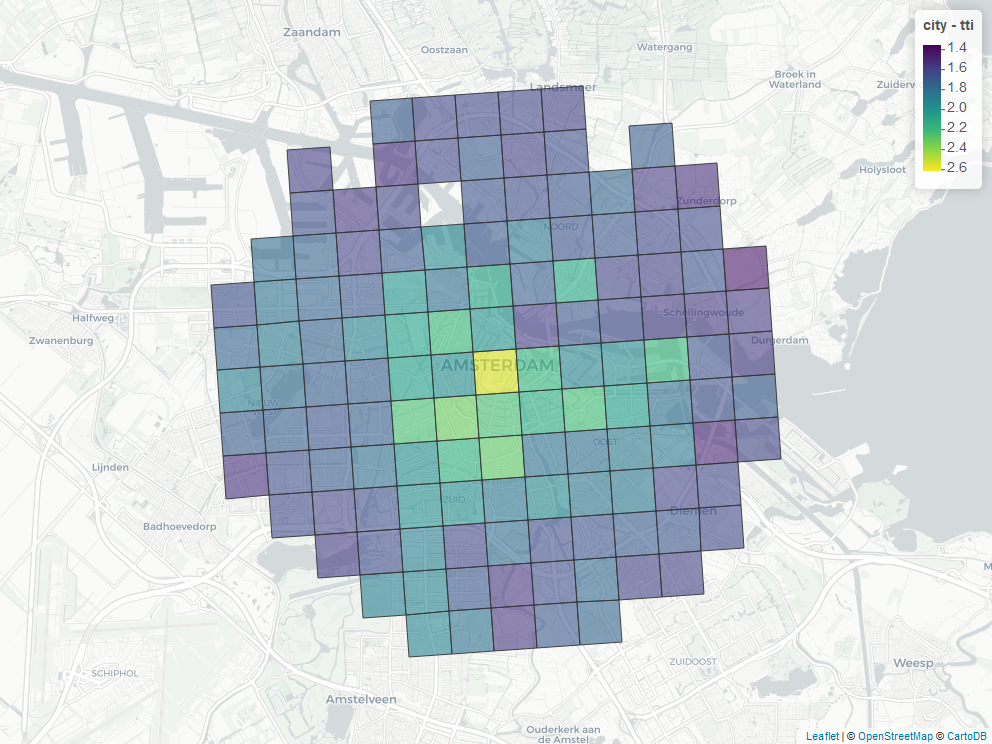
\includegraphics[width=0.8\linewidth, height=4cm]{./Img/amsterdam_tti}} \par 
			%
			\subfloat[Glasgow]{\centering
				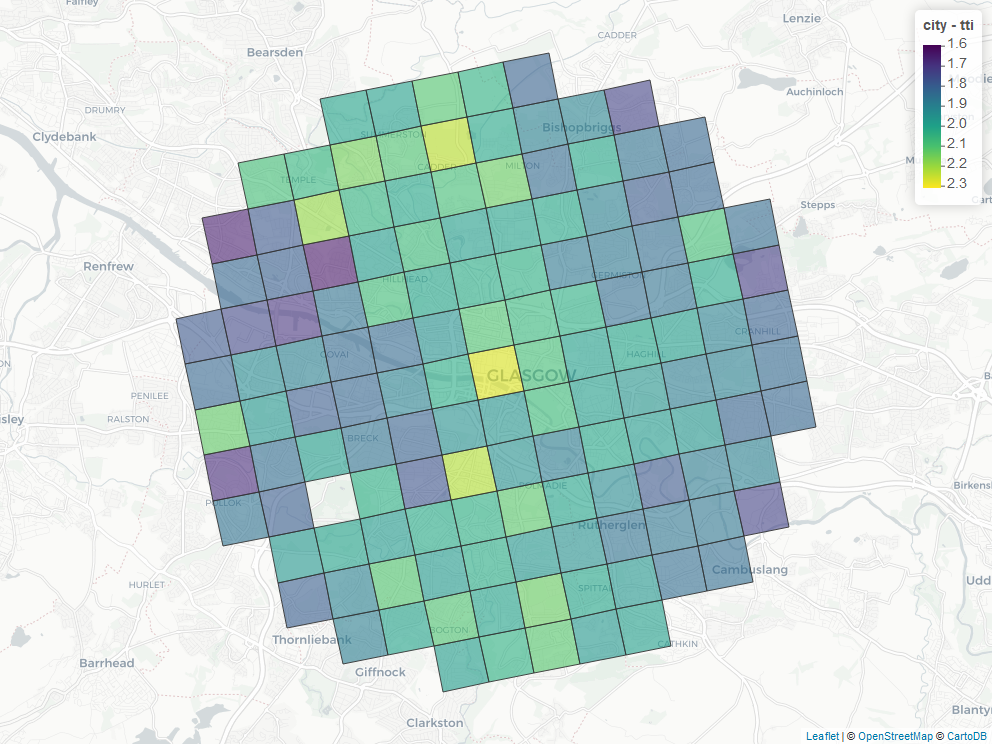
\includegraphics[width=0.8\linewidth,height=4cm]{./Img/glasgow_tti}} \newpage
			%
			\subfloat[Goteborg]{\centering
				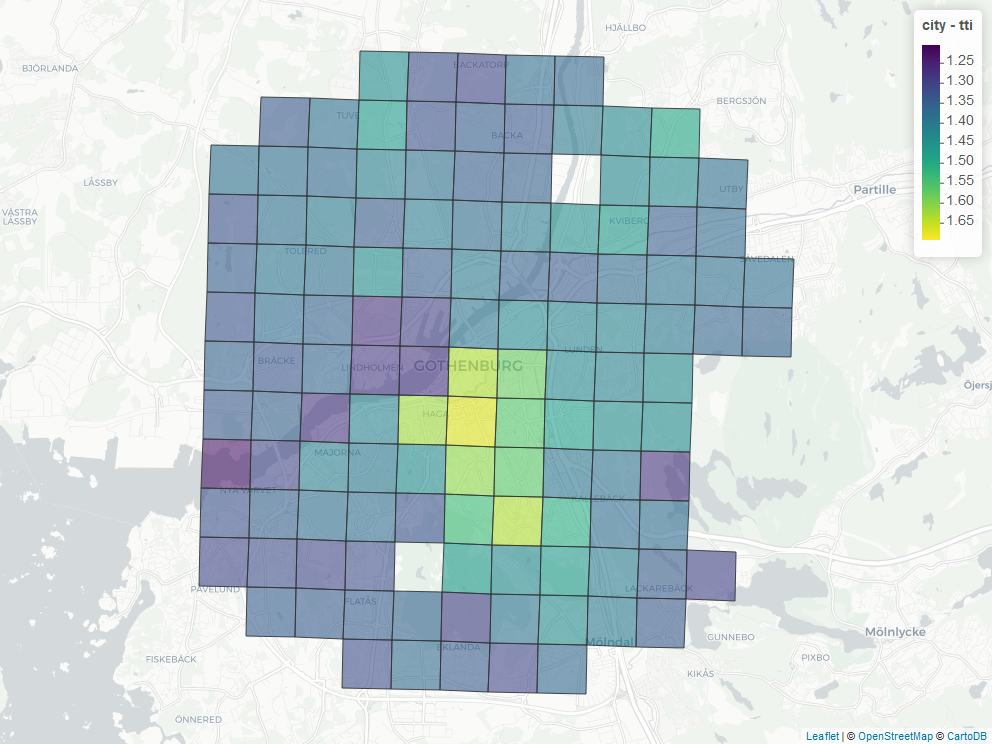
\includegraphics[width=0.8\linewidth,height=4cm]{./Img/goteborg_tti}} \par
			%
			\subfloat[Lisbon]{\centering
				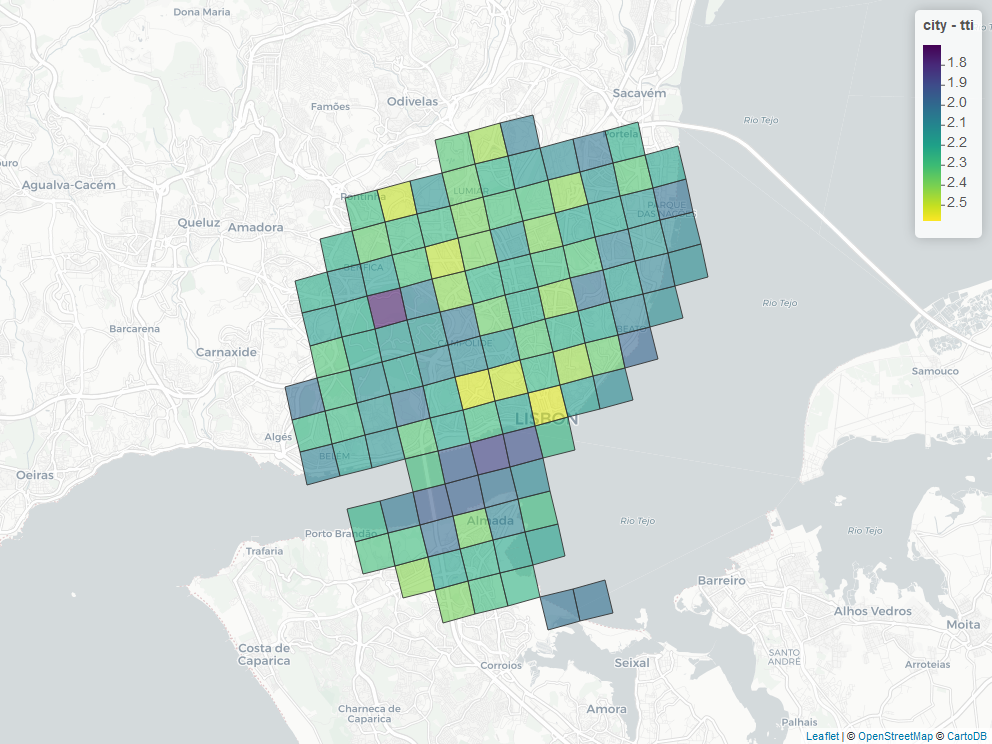
\includegraphics[width=0.8\linewidth, height=4cm]{./Img/lisbon_tti}} \par
			%	
		\end{multicols}
		\caption{Images extracted from results}
		\label{fig:result_tti}
	\end{figure}
	
	
	\begin{figure}[H]
		\centering
		\begin{multicols}{2}
			\noindent
			%
			\subfloat[Amsterdam]{\centering
				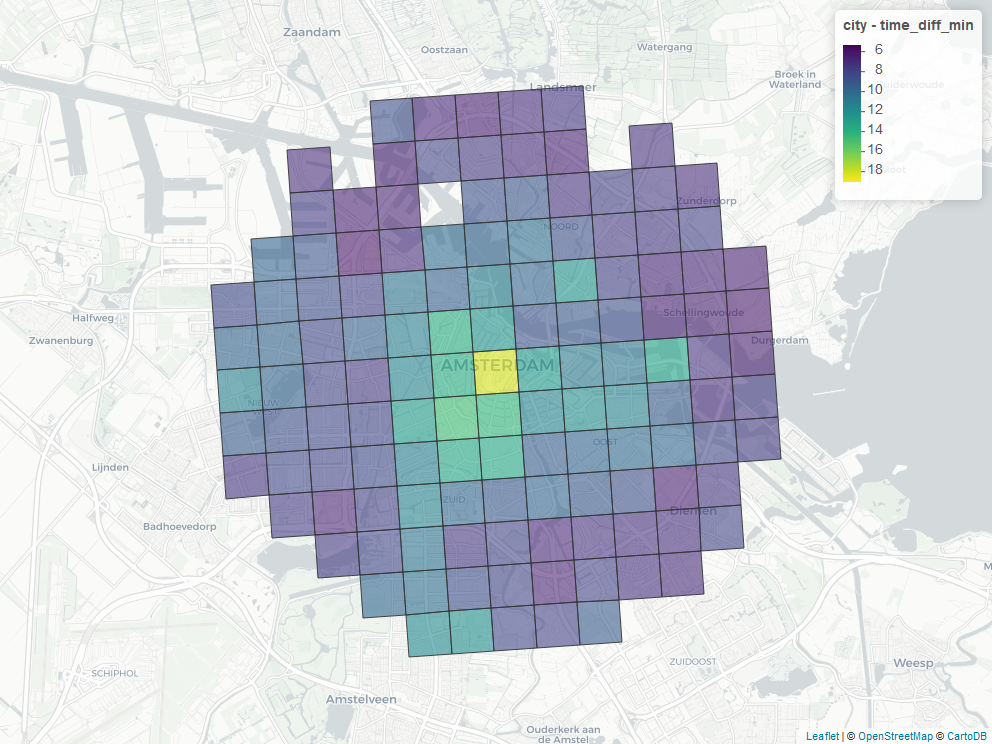
\includegraphics[width=0.8\linewidth, height=4cm]{./Img/amsterdam_time_diff_min}} \par 
			%
			\subfloat[Glasgow]{\centering
				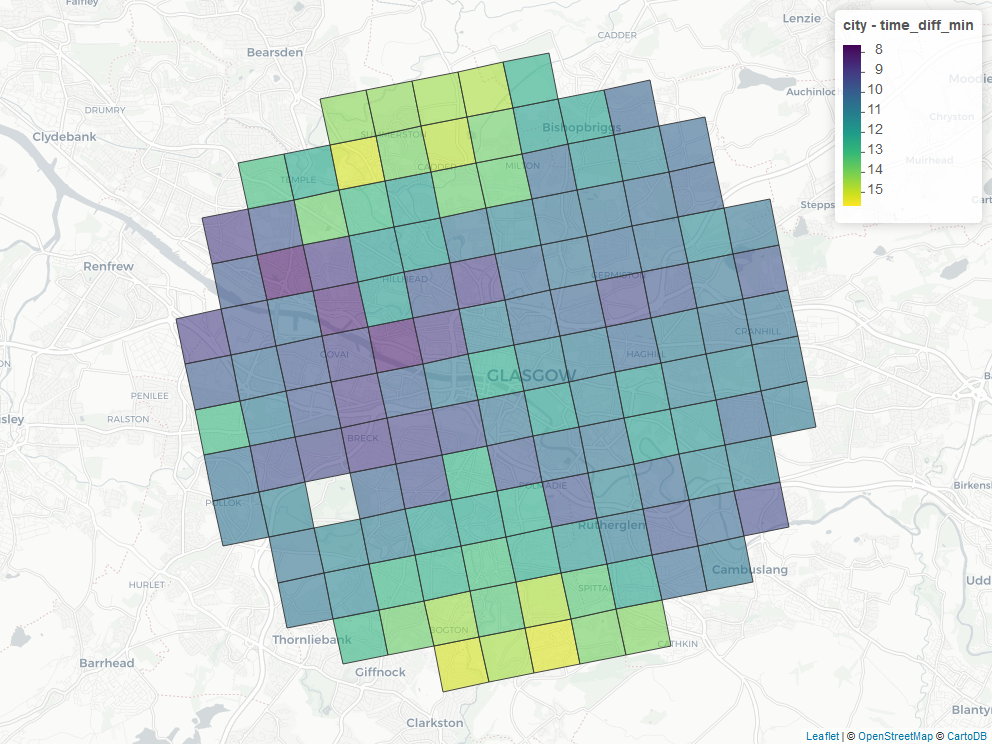
\includegraphics[width=0.8\linewidth,height=4cm]{./Img/glasgow_time_diff_min}} \newpage
			%
			\subfloat[Goteborg]{\centering
				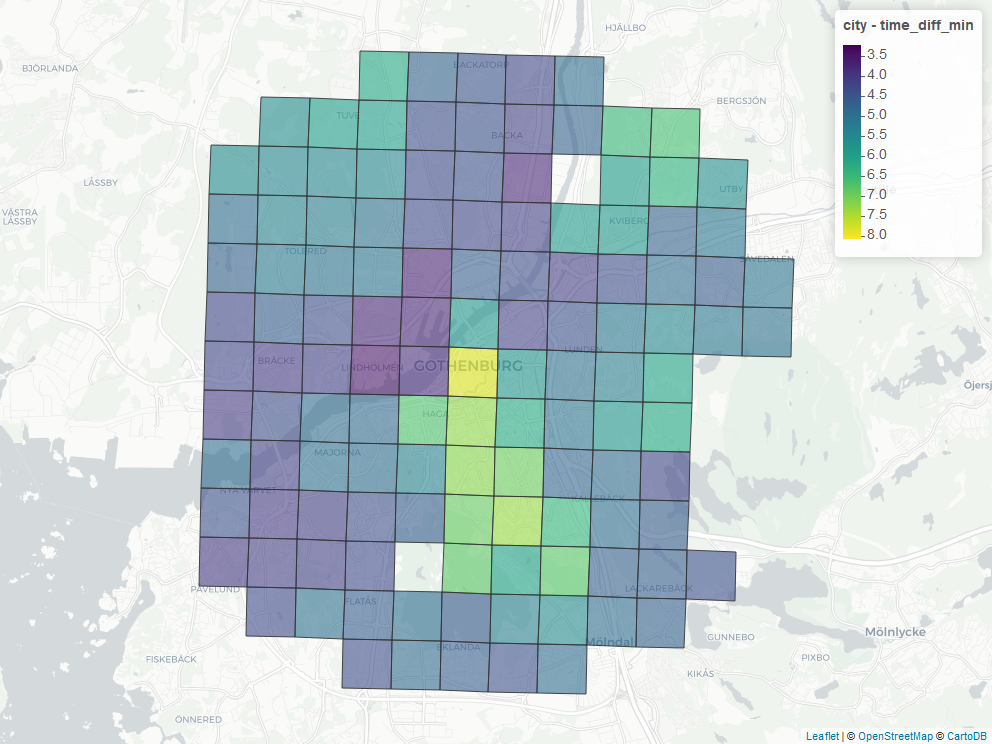
\includegraphics[width=0.8\linewidth,height=4cm]{./Img/goteborg_time_diff_min}} \par
			%
			\subfloat[Lisbon]{\centering
				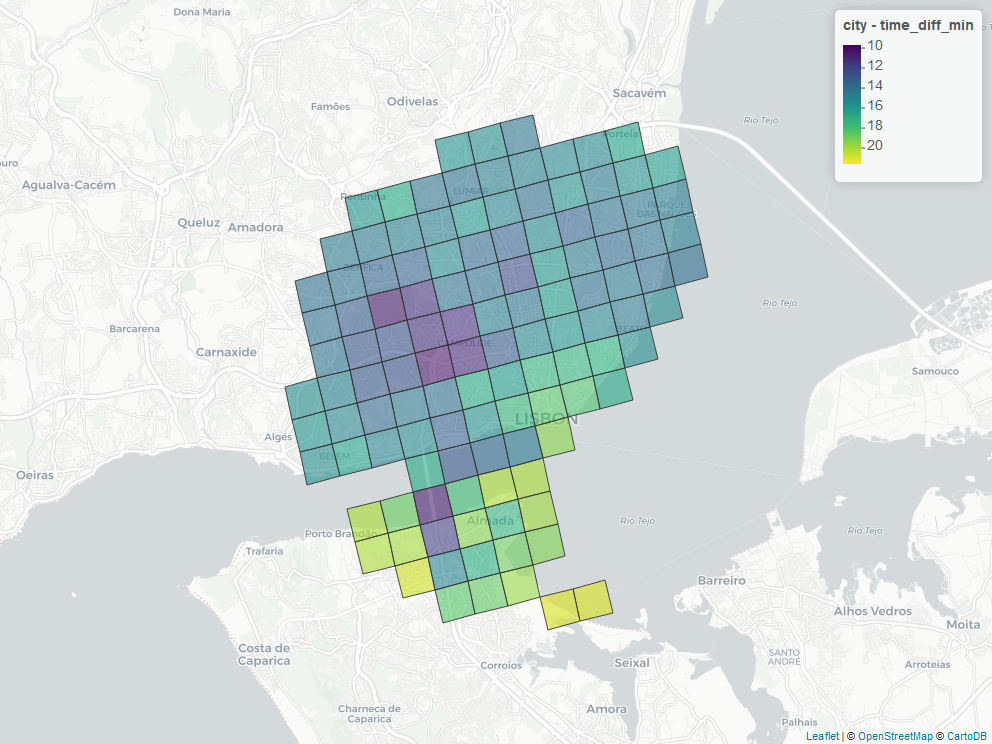
\includegraphics[width=0.8\linewidth, height=4cm]{./Img/lisbon_time_diff_min}} \par
			%	
		\end{multicols}
		\caption{Images extracted from results}
		\label{fig:result_diff}
	\end{figure}
	
	
	%%%%%%%%%%%%%%%%%%%%%%%%%%%%%%%%%%%%%%%%%%%%%%%%%%%%%%%%%%%%%%%%%%%%%%%%%
	\section{Discussion} %%%%%%%%%%%%%%%%%%%%%%%%%%%%%%%%%%%%%%%%%%%%%%%%%%%
	%%%%%%%%%%%%%%%%%%%%%%%%%%%%%%%%%%%%%%%%%%%%%%%%%%%%%%%%%%%%%%%%%%%%%%%%%
	The methodology presented in this paper exploits a new data source to provide spatial insights about traffic congestion in different cities. The information generated allows planning and transport agencies to reconstruct some of the most popular indexes discussed in the theoretical background section.\par
	
	% Validation
	In order to determine the validity of the methodology presented here, the aggregated results were compared against the results published by two internationally recognized companies which offer transportation solutions. With different business models, INRIX, HERE and TomTom in the last years started to offer transportation insights as a service. Historically, INRIX has been consulted to provide he levels of congestion in several countries in the OECD and U.S. transport agencies \parencite{Eurostat2016, TheTexasA&MTransportationInstitute2019}, but given the increase in the amount of devices embedded with GPS, other businesses have found them self in a position of exploiting these new data sources. Nowadays, they all offer transportation consulting services. \textcite{Inrix2018} and \textcite{TomTom2018} publish results on traffic congestion and rank cities according to different criteria. For instance INRIX reports the amount of hours lost in congestion, the cost per driver, travel time and speed whereas TOMTOM shows a congestion percentage. Although, is difficult to compare across these indicators, if the ranking of cities is taken into account the methodology presented here, along with TomTom and INRIX, position Goteborg as the least congested, followed by Amsterdam, Glasgow and finally Lisbon. It is relevant to highlight that, INRIX and TomTom provide more detailed information for each city, but no maps are found and the spatial distribution of the problem remains unknown. \par
	
	This process was not conceived to show congestion levels at street level, but to identity areas which area affected by this phenomena. Transport or planning practitioners interested in getting traditional information about levels of service, will not find answers by applying this methodology. \par 
	
	%Importance of maps
	Traffic congestion deteriorate different domains of urban life and as a consequence the focus on the problem varies across disciplines. \textit{'Throughout the world, traffic congestion reduces the core benefit of cities: the ability to connect with other people easily'} \parencite{Glaeser2011}, so it becomes crucial to understand who suffers from congestion the most and what parts of the city are more vulnerable to the problem. Therefore looking at the congestion level of street segments is useful for traffic planning, but insufficient to solve broader issues. \par
	
	The maps of congestion produced as a result of applying this methodology directly establish the relationship between a population living in an area and the level of congestion faced. \par
	
	% Over time
	When dealing with city planing, it is difficult to understand how an urban intervention or policy affects the rest of the city.This approach can be iterated over time, to see how transport congestion evolves over time and evaluate to what extent certain policies are being effective in changing traffic congestion patterns.\par
	
	
	\subsection{Limitations and future work}%%%%%%%%%%%%%%%%%%%%%%%%%%%%%%%%
	%%%%%%%%%%%%%%%%%%%%%%%%%%%%%%%%%%%%%%%%%%%%%%%%%%%%%%%%%%%%%%%%%%%%%%%%
	The methodology presented in this study relays primarily in Google's web service and this fact is a drawback as users have no control over the service standards, usability or costs. For instance, the type request performed during this study had a cost of 10 U\$D/1000 requests, considering a grid of 100 cells, will generate 9,900 travel routes and to estimate congestion a total of 19,800 requests will be needed. This process will involve a cost of 198 U\$D and almost to hours to complete. Consequently, before considering expanding the study to cover more cities, take into consideration extensive metropolitan areas or repeating the process for different moments, budget constraints must be taken into consideration. \par
	The results presented here, took the EuroStat population 1km2 grid cell to retrieve traffic information. Certainly, this decision was arbitrary and the shape/size of these areas can be subject of debate. Although, to map the historical city center this representation is to big, it make sense for planning and data purchase became affordable.\par
	
	Nevertheless, the zones used for the analysis can be easily interchanged with other geographical representations, allowing the process to be enriched in several dimensions. Census tracks with socio-economic information could be used to refine the method, the amount of cars or age groups could help to better understand to what degree this citizens are affected and to explore whether there is a relation between car use and congestion levels. Moreover, an origin and destination survey with geographical zones can be used used in the study to weight the different desire lines of travel. Depending on the characteristics of each data source, this methodology can be expanded and refined in different manners.\par
	
	The results presented here, do not necessarily imply that \textit{'more congested'} places are demanding for solutions from public administration, but attention. \textit{'Traffic problems'} can be the result of poor infrastructure, an excess of demand or a combination of both. The method only reflects time delays faced by private commuting and in some cases, such as in city centres, this can be a desirable tool to demotivate car use. \par
	
	Google API also offers estimations for public transport, that can be used provide a more comprehensive estimation of how congestion by different transport modes. \par
	
	Finally, but not least this work presents one alternative of how synthetic data can be used to provide new insights. The method only uses a dull origin and destination matrix with modelled traffic information. Traditional data sources such as population census or travel survey could be combined to update or generate richer data sets. In this case, the population grid was used because it would eventually allow to weight the results obtained and give relative importance to different zones based on population. Travel surveys, with information about time, commuting modes, car type and specific origins and destinations could be used to feed this methodology to model precisely how much GHGs are being emitted and bench-marked under \textit{non-congested scenarios.} \par
	
	
	
	
	
	
	%%%%%%%%%%%%%%%%%%%%%%%%%%%%%%%%%%%%%%%%%%%%%%%%%%%%%%%%%%%%%%%%%%%%%%%%
	\section{Conclusion} %%%%%%%%%%%%%%%%%%%%%%%%%%%%%%%%%%%%%%%%%%%%%%%%%%%
	%%%%%%%%%%%%%%%%%%%%%%%%%%%%%%%%%%%%%%%%%%%%%%%%%%%%%%%%%%%%%%%%%%%%%%%%
	The study presented a methodological approach to study the how traffic congestion is spatially distributed within an urban area. Generating a synthetic Origin-Destiny matrix, the method uses an online routing service to estimate different travel routes. The methodology provides a non-expensive, generalizable and systematic to estimate congestion in different parts of a city. The data retrieved can be mapped, thus used by city planners and transportation agencies. The aggregation of the data provide conclusions that are consistent with internationally recognized institutions such as INRIX and TomTom. 
	
	
	%%%%%%%%%%%%%%%%%%%%%%%%%%%%%%%%%%%%%%%%%%%%%%%%%%%%%%%%%%%%%%%%%%%%%%%%
	\printbibliography %%%%%%%%%%%%%%%%%%%%%%%%%%%%%%%%%%%%%%%%%%%%%%%%%%%%%
	%%%%%%%%%%%%%%%%%%%%%%%%%%%%%%%%%%%%%%%%%%%%%%%%%%%%%%%%%%%%%%%%%%%%%%%%
	
	
\end{document}








